%%%%%%%%%%%%%%%%%%%%%%%%%%%%%%%%%%%%%%%%%%%%%%%%%%%%%%%%%%%%%%%%%%%%%%%%%%
%
% 	Template for seminar reports
%
%%%%%%%%%%%%%%%%%%%%%%%%%%%%%%%%%%%%%%%%%%%%%%%%%%%%%%%%%%%%%%%%%%%%%%%%%%

\documentclass[a4paper,pdftex]{scrartcl}

\usepackage[utf8]{inputenc}

% graphicx and figures
\usepackage{graphicx}
\usepackage{float}
\usepackage{caption}
\usepackage{subcaption}

% C code
\usepackage{listings}

% url
\usepackage[hyphenbreaks]{breakurl}
\usepackage[hyphens]{url}

\begin{document}

%%%%%%%%%%%%%%%%%%%%%%%%%%%%%%%%%%%%%%%%%%%%%%%%%%%%%%%%%%%%%%%%%%%%%%%%%%
% 	Paper title
%%%%%%%%%%%%%%%%%%%%%%%%%%%%%%%%%%%%%%%%%%%%%%%%%%%%%%%%%%%%%%%%%%%%%%%%%%
\title{Introduction to LBM}
\subtitle{Seminar Lattice Boltzmann Methods:\\Theory, Implementation and Applications}

\author{
Denys Korzh\\
Department of Computational Science and Engineering\\Technische Universit\"at M\"unchen\\
Email: denys.korzh@tum.de 
}

\maketitle

% include abstract

\begin{abstract}
Lattice-Boltzmann method (LBM) is a good example of developing new approaches in science. As a relatively young computational fluid dynamics (CFD) method it already has many different implementations and it is a factor in the automotive industry. The advantage of LBM over other conventional CFD methods is in dealing with complex boundaries, incorporating microscopic interactions, and good parallelization of the algorithm.
\end{abstract}

% no page number on first page
\thispagestyle{empty}
%%%%%%%%%%%%%%%%%%%%%%%%%%%%%%%%%%%%%%%%%%%%%%%%%%%%%%%%%%%%%%%%%%%%%%%%%%
% 	Sections, Subsections,...
%%%%%%%%%%%%%%%%%%%%%%%%%%%%%%%%%%%%%%%%%%%%%%%%%%%%%%%%%%%%%%%%%%%%%%%%%%


\section{Introduction}

Lattice-Boltzmann method is an approach to implement fluid flows. LBM is based on statistical physics, in contrast to Navier-Stocks approach (NS), which discretizes Navier-Stocks equations and solves them directly.

LBM belongs to Mesoscale as opposed by NV (Macroscale) and Molecular Dynamics (Microscale). LBM is a simplification (abstraction) of Molecular Dynamics (MD) and NS is an averaging of LBM. Results obtained with NS approach (vector field, density, pressure) can be computed from LBM results.

The Lattice-Boltzmann method was developed in 1988 by G. McNamara and G. Zanetti [2], making it a relatively new method that still undergoes dynamical development.

This paper consists of 7 sections. In first two sections we will introduce  Lattice-Boltzmann method and tell the history of LBM development. From third to sixth section the concepts of the method, and their  implementation, will be presented. And the  summary will be the last part of the paper.

\subsection{Advantage over NSE}

NS equations (NSE) describe flow only for incompressible, isothermal, Newtonian fluid. It assumes a continuum domain. Not all problems can be solved with NSE (e.g. carbon nanotube flows). Fluids in reality are composed of atoms and molecules, which have empty space in between. Fluids under the continuum assumption are composed of continuous matter, filling the entire space. Continuum assumption is valid for $Kn \ll 1$ where Kn is a Knudsen number:
\begin{equation}
Kn=\frac{\lambda}{L_c},
\end{equation}
where $L_c$ is a characteristic length and $\lambda$ - mean free path. Air has $\lambda \approx O(nm)$ in STP(Standard conditions for temperature and pressure).

If we have a small particle in a fluid at rest then the velocity of the particle $U=0$, $L_c$ is equal to the diameter of the particle which decreases, thereby increasing $Kn$ and when $Kn$ approaches 1, the particle begins to feel collisions with individual molecules, resulting in Brownian motion. However, it should be noted that NSE does not predict individual motions of particles.

\subsection{Advantage over Molecular Dynamics}

The downside of using MD simulations is its extreme restrictions on the memory size. The largest MD simulation is $4.125\times 10^{12}$ particles [4] — for comparison, one millilitre of water consists of $3\times 10^{22}$ particles.


\section{Cellular automata}
In LGCA we have different restrictions which simplifies our computations and decrease the computation costs, in comparison to MD. For example molecule-to-molecule forces are replaced with rigid body collisions, and during one time step, particles can travel only along one edge.  The velocities are discretized too, what implies that all particles have the same energy and at the end of a time step particles can reside only at vertices.
The first lattice-gas cellular automata (LGCA) was proposed in 1973 by Hardy, de Pazzis and Pomeau [3]. It is named HPP and is a CA model over square lattice. HPP does not lead to Navier-Stokes equations, because of insufficient degree of rotational symmetry of the lattice. But still it worth of discussion, and we will do it later on.

Frish-Hasslacher-Pomeau is the model of LGCA (see Fig. 1), which lead to Navier-Stokes equations, because of it's symmetry. For example Frish-Hasslacher-Pomeau automata has following prescriptions [2]:

\begin{itemize}
\item All particles have the same mass m=1.
\item Particles can move only along one of the six directions defined by the discrete displacements $c_{i}$.
\item In a time-cycle (made one for convenience) the particles hop to the neares neighbor pointed by the corresponding discrete vector $c_{i}$. Both longer and shorter jumps are forbidden which means all lattice particles have the same energy.
\item No two particles sitting on the same site can move along the same direction $c_{i}$ (exclusion principle).
\end{itemize}

\begin{figure}[H]
  \centering
  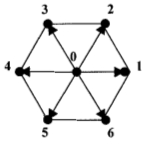
\includegraphics[width=0.1\textwidth]{img/fig1.png}
  \caption{The FHP hexagonal lattice [2].}
\end{figure}

In LGCA we have such basic mechanisms:

\begin{itemize}
\item Free-streaming: $ n_i^{in}(\vec{r}+\vec{c}_{i}\Delta t, t+\Delta t) = n_i^{out}(\vec{r}, t) $
\item Collision: $ n_i^{out}(\vec{r}, t) = n_i^{in}(\vec{r}, t) + \Omega(n_i^{in}(\vec{r}, t)) $.
\end{itemize}
Where $\Omega$ is a collision operator.

Free-streaming is a simple transfer of particles according of their discrete velocities.

When two particles meet each other on the site they interact and exchange their momenta following the discretization rules of the lattice. Such exchange is called collision. In HPP only two particles can collide, that is why the collision in HPP is deterministic(see Fig. 2 (a)).

If we will consider the collision of two particles in FHP, then we will have non-deterministic outcome(see Fig. 2 (b)).


\begin{figure}[H]
  \centering
  \begin{subfigure}[h]{0.5\textwidth}
    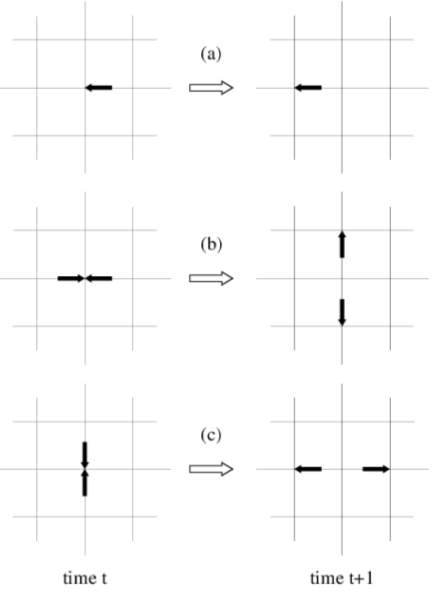
\includegraphics[width=\textwidth]{img/fig4.png}
    \caption{HHP streaming(a)/collision(b,c) [6].}
  \end{subfigure}
  \begin{subfigure}[h]{0.3\textwidth}
    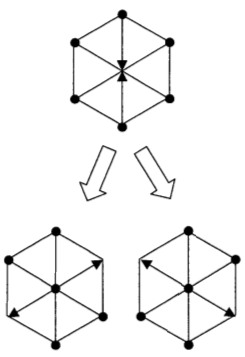
\includegraphics[width=\textwidth]{img/fig5.png}
    \caption{FHP collision [2].}
  \end{subfigure}
  \caption{Collision of two particles / streaming.}
\end{figure}

Albeit all restrictions this collision shares two crucial features such as conversation of particle number and conversation of the total momentum.

\begin{itemize}
\item conserve mass (number of particles): $ \sum_i n_i^{in} = \sum_i n_i^{out} $
\item conserve momentum: $ \sum_i n_i^{in} \vec{c}_{ia} = \sum_i n_i^{out} \vec{c}_{ia} $
\end{itemize}

The exclusion principle is kept too. There are no two particles with the same position and velocity at the same time.

One of the biggest advantages of LGCA is it's easy implementation, and  the easiness of it's parallelization, because of locality behaviour of the collision operator.

But the discretization works not always. For Macro-view such discretization is not a big problem, because we always discretize, but for Micro-view such restrictions can bring to huge inconsistency and very poor precision. Restriction in velocity direction and magnitude cannot describe model on microscopic level. In LGCA includes state of particle where the velocity is equal to zero(stationary particles), but in real word of microscopic level there can not exist such particles. There several main drawbacks of LGCA, but the most important one is statistical noise.

Lattice-Boltzmann approach was created as a respond on the main problems of LGCA, using an statistical averaging procedure.



\section{Statistical mechanics}

The basic idea of the Lattice-Boltzmann equations is to replace Boolean occupation numbers $n_i$ in LGCA with the corresponding ensemble-averaged populations. It can be shown, that the Boltzmann equation

\begin{equation}
\frac{\partial f}{\partial t} + \vec{v} \nabla f = Q
\end{equation}

can be referred to LGCA discrete kinetic equation

\begin{equation}
n_i(\vec{x} + \vec{c}_i \Delta t, t + \Delta t) = n_i(\vec{x},t) +\Delta_i
\end{equation}

by expansion of the left hand side

\begin{equation}
n_i(\vec{x} + \vec{c}_i \Delta t, t + \Delta t) = n_i(\vec{x},t) + \Delta t \frac{\partial n_i}{\partial t} + \vec{c}_i \Delta{t} \nabla{n_i} + O\big(\Delta t)^2\big).
\end{equation}
Neglecting higher order terms, one obtains
\begin{equation}
\frac{\partial n_i}{\partial t} + \vec{c}_i \nabla{n_i} = \frac{\Delta_i}{\Delta t}
\end{equation}
and if the following  substitutions are done, $n_i \rightarrow f$, $\vec{c}_i \rightarrow \vec{v}$, $\frac{\Delta_i}{\Delta t} \rightarrow Q$, then the approximation of the Boltzmann equation will be obtained. Q collision integral is very complex and is very complicated to compute, that is why it was proposed to replace it with BGK (Bhatnagar-Gross-Krook) approximation

\begin{equation}
\frac{\partial f}{\partial t} + \vec{v} \nabla f = -\frac{1}{\tau}(f - f^{(eq)}),
\end{equation}
where $f^{eq}$ is a Maxwell-Boltzmann equilibrium distribution. The idea behind BGK is that our model should follow Maxwell–Boltzmann distribution law, and the difference inside of collision operator gives us the deviation of computed $f$ from Maxwell Boltzmann equilibrium distribution.

In the end the  Boltzmann equations are discretized to obtain Lattice-Boltzmann method
\begin{equation}
f_i(\vec{x} + \vec{c}_i \Delta t, t + \Delta t) = f_i(\vec{x},t) + -\frac{1}{\tau} \big(f_i(\vec{x},t) - f_i^{(eq)}(\rho(\vec{x},t), u(\vec{x},t))\big)
\end{equation}
where $\rho$ and $u$ are macroscopic density and velocity of the flow. As one can see, instead of using the occupation number $n_i$ the distribution functions $f_i$ is used, which basically removes the LGCA noise. Equation (7) is actually a collision update step in the LBM.

For the lattice BGK model, the equilibrium distribution function can be calculated as

\begin{equation}
f_i^{(eq)} = f_i^{(eq)}(\rho, u) = t_p \rho ( 1 + \frac{3}{c^2} c_i u + \frac{9}{2c^4} (c_i u)^2 - \frac{3u^2}{2c^2})
\end{equation}
where $c_i$ is the corresponding lattice velocity, $c$ is the velocity of sound and $t_p$ is a direction dependent parameter, which depends on DdQq model, where d is the number of dimensions and q is the number of directions in which velocities are discretized.

In case of the D2Q9 model, $t_p$ can be derived as

\begin{equation}
t_p = \frac{4}{9} \quad \textrm{for} \quad ||c_i||=0
\end{equation}
\begin{equation}
t_p = \frac{1}{9} \quad \textrm{for} \quad ||c_i||=1
\end{equation}
\begin{equation}
t_p = \frac{1}{36} \quad \textrm{for} \quad ||c_i||=\sqrt{2}
\end{equation}
and in case of the D3Q19 model as

\begin{equation}
t_p = \frac{1}{3} \quad \textrm{for} \quad ||c_i||=0
\end{equation}
\begin{equation}
t_p = \frac{1}{18} \quad \textrm{for} \quad ||c_i||=1
\end{equation}
\begin{equation}
t_p = \frac{1}{36} \quad \textrm{for} \quad ||c_i||=\sqrt{2}
\end{equation}

For both the D2Q9 and the D3Q19 model, the parameter $c$ can be considered to be 1.


\section{Statistical mechanics}

The basic idea of LBE is to replace Boolean occupation numbers $n_i$ in LGCA with the corresponding ensemble-averaged populations. It can be shown, that Boltzmann equation

\begin{equation}
\frac{\partial f}{\partial t} + \overrightarrow{v} \nabla f = Q
\end{equation}

can be referred to LGCA discrete kinetic equation

\begin{equation}
n_i(\overrightarrow{x} + \overrightarrow{c}_i \Delta t, t + \Delta t) = n_i(\overrightarrow{x},t) +\Delta_i
\end{equation}

by expansion of the left hand side

\begin{equation}
n_i(\overrightarrow{x} + \overrightarrow{c}_i \Delta t, t + \Delta t) = n_i(\overrightarrow{x},t) + \Delta t \frac{\partial n_i}{\partial t} + \overrightarrow{c}_i \Delta{t} \nabla{n_i} + O\big(\Delta t)^2\big)
\end{equation}
and if we will substitute $n_i \rightarrow f$, $\overrightarrow{c}_i \rightarrow \overrightarrow{v}$, $\frac{\Delta_i}{\Delta t} \rightarrow Q$, then we will get Boltzmann equation. Q collision integral is very complex and is very complicated to compute, that is why it was proposed to replace it with BGK (Bhatnagar-Gross-Krook) approximation

\begin{equation}
\frac{\partial f}{\partial t} + \overrightarrow{v} \nabla f = -\frac{1}{\tau}(f - f^{(eq)})
\end{equation}
Where $f^{eq}$ is Maxwell Boltzmann equilibrium distribution. The idea behind BGK is that our model should follow Maxwell–Boltzmann distribution law, and the difference inside of collision operator gives us the deviation of computed $f$ from  Maxwell Boltzmann equilibrium distribution.

At the end we discretize Boltzmann equations to get Lattice-Boltzmann method

\begin{equation}
f_i(\overrightarrow{x} + \overrightarrow{c}_i \Delta t, t + \Delta t) = f_i(\overrightarrow{x},t) + -\frac{1}{\tau} \big(f_i(\overrightarrow{x},t) - f_i^{(eq)}(\rho(\overrightarrow{x},t), u(\overrightarrow{x},t))\big)
\end{equation}
where $\rho$ and $u$ are macroscopic density and velocity of the flow.

For the lattice BGK model, the equilibrium distribution function can be calculated as

\begin{equation}
f_i^{(eq)} = f_i^{(eq)}(\rho, u) = t_p \rho ( 1 + \frac{3}{c^2} c_i u + \frac{9}{2c^4} (c_i u)^2 - \frac{3u^2}{2c^2})
\end{equation}
where $c_i$ is the corresponding lattice velocity, $c$ is the velocity of sound and $t_p$ is a direction dependent parameter, which depends on DdQq model. Where d is the number of dimensions and q is the number of directions in which velocities are discretized.

In case of the D2Q9 model, $t_p$ can be derived as

\begin{equation}
t_p = \frac{4}{9} \quad \textrm{for} \quad ||c_i||=0
\end{equation}
\begin{equation}
t_p = \frac{1}{9} \quad \textrm{for} \quad ||c_i||=1
\end{equation}
\begin{equation}
t_p = \frac{1}{36} \quad \textrm{for} \quad ||c_i||=\sqrt{2}
\end{equation}
and in case of the D3Q19 model as

\begin{equation}
t_p = \frac{1}{3} \quad \textrm{for} \quad ||c_i||=0
\end{equation}
\begin{equation}
t_p = \frac{1}{18} \quad \textrm{for} \quad ||c_i||=1
\end{equation}
\begin{equation}
t_p = \frac{1}{36} \quad \textrm{for} \quad ||c_i||=\sqrt{2}
\end{equation}

For both the D2Q9 and the D3Q19 model, the parameter $c$ can be considered to be 1.


\section{Simple boundary conditions}

Any fluid flow model cannot be build without including of the influence of the surrounding environment. This influence can be described mathematically with so called boundary conditions. If the boundary conditions are not set, then at the end all the probability densities will be streamed out of the domain with the streaming step. Boundary conditions build the external constraints which influence the solution of the whole system. The implementation of the boundary conditions in LBM is straightforward, but the mathematical background of these boundary conditions may be even more complicated than the LBM itself.

One of the easiest boundary conditions is a no-slip (see Fig. \ref{fig:no-slip-BC}). The no-slip boundary conditions are used in case of real walls or obstacles, which offer a certain amount to friction of the fluid. In the case when the fluid velocity at the wall is reduced to zero, the boundary conditions can be implemented in the following way: all distribution functions of a fluid cell neighboring an obstacle cell pointing towards the obstacle are simply reversed \cite{pflaum}. This assures that the fluid velocity normal and tangential to the wall are zero. These are so called Dirichlet boundary conditions.

\begin{figure}[H]
  \centering
  \begin{subfigure}[h]{0.3\textwidth}
    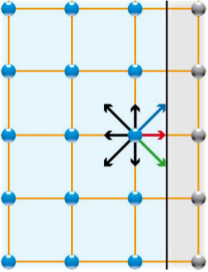
\includegraphics[width=\textwidth]{img/fig8-1.png}
  \end{subfigure}
  \begin{subfigure}[h]{0.3\textwidth}
    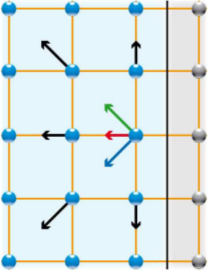
\includegraphics[width=\textwidth]{img/fig8-2.png}
  \end{subfigure}
  \caption{No-slip boundary conditions. Left - before streaming step; Right – after streaming step \cite{pflaum}.}\label{fig:no-slip-BC}
\end{figure}

The next simple boundary conditions are free-slip boundary conditions (see Fig. \ref{fig:free-slip-BC}). They can be used if there are walls without friction. A usual example of free-slip boundary conditions is at symmetry axes in certain simulation domains, for example in the middle of a channel flow. The free-slip boundary conditions are applied as follows: all distribution functions of a fluid cell neighboring a free-slip boundary pointing towards the boundary are reflected in their component normal to the wall. This assures that the velocity normal to the wall is zero, whereas the velocity tangential to the wall remains unchanged \cite{pflaum}. These are so called Neumann boundary conditions:

\begin{equation}
\frac{\partial v_t}{\partial n} = 0.
\end{equation}

\begin{figure}[H]
  \centering
  \begin{subfigure}[h]{0.3\textwidth}
    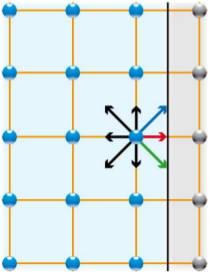
\includegraphics[width=\textwidth]{img/fig9-1.png}
  \end{subfigure}
  \begin{subfigure}[h]{0.3\textwidth}
    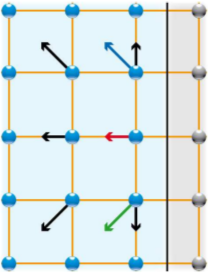
\includegraphics[width=\textwidth]{img/fig9-2.png}
  \end{subfigure}
  \caption{Free-slip boundary conditions. Left - before streaming step; Right – after streaming step \cite{pflaum}.}\label{fig:free-slip-BC}
\end{figure}

To implement the lid-driven cavity, which will be described in the next section, more boundary conditions are needed. Such boundary conditions are called bounce-back condition with additional acceleration (see Eq. 21) and used to model a moving wall. With such boundaries there is a wall that moves with some certain velocity, which is imparted to the fluid particles, accelerating the fluid. These boundaries are similar to no-slip boundaries except for the scaling term depending on the wall velocity \cite{pflaum}:

\begin{equation}
f_{\bar{\alpha}}(\vec{x},t) = f_{\alpha}(\vec{x},t) - 2 t_p \rho \frac{3}{c^2} c_{\alpha} u_{w}
\end{equation}
where $\alpha$ is the direction towards the wall, $\bar{\alpha}$ is the reverse direction from the wall, $t_p$ is the direction dependent parameter, $\rho$ is the fluid density of the near wall fluid cell, and $u_w$ is the wall velocity.



\section{Own implementation: lid-driven cavity}

In my own implementation [5] I implemented lid-driven cavity in 3D with D3Q19 model. The streaming and collision were implemented as described before in two different steps. Further figures are received on the 5000th iteration. The initial velocity of the lid was 0.01 and the size of the cavity was 50 cells. On the figure 7 you can see density distribution. In both corners of the cavity you can observe high and low density zones which response to hight and low pressure respectively. Which is correct case, when you simulate lid-driven cavity.

The resulted velocities you can see on the figure 8. In the left lower corner is the vertex which response to the stream with direction other then main vertex, what response to the result if you simulate lid-driven cavity with Navier-Stokes equations.

\begin{figure}[H]
  \centering
  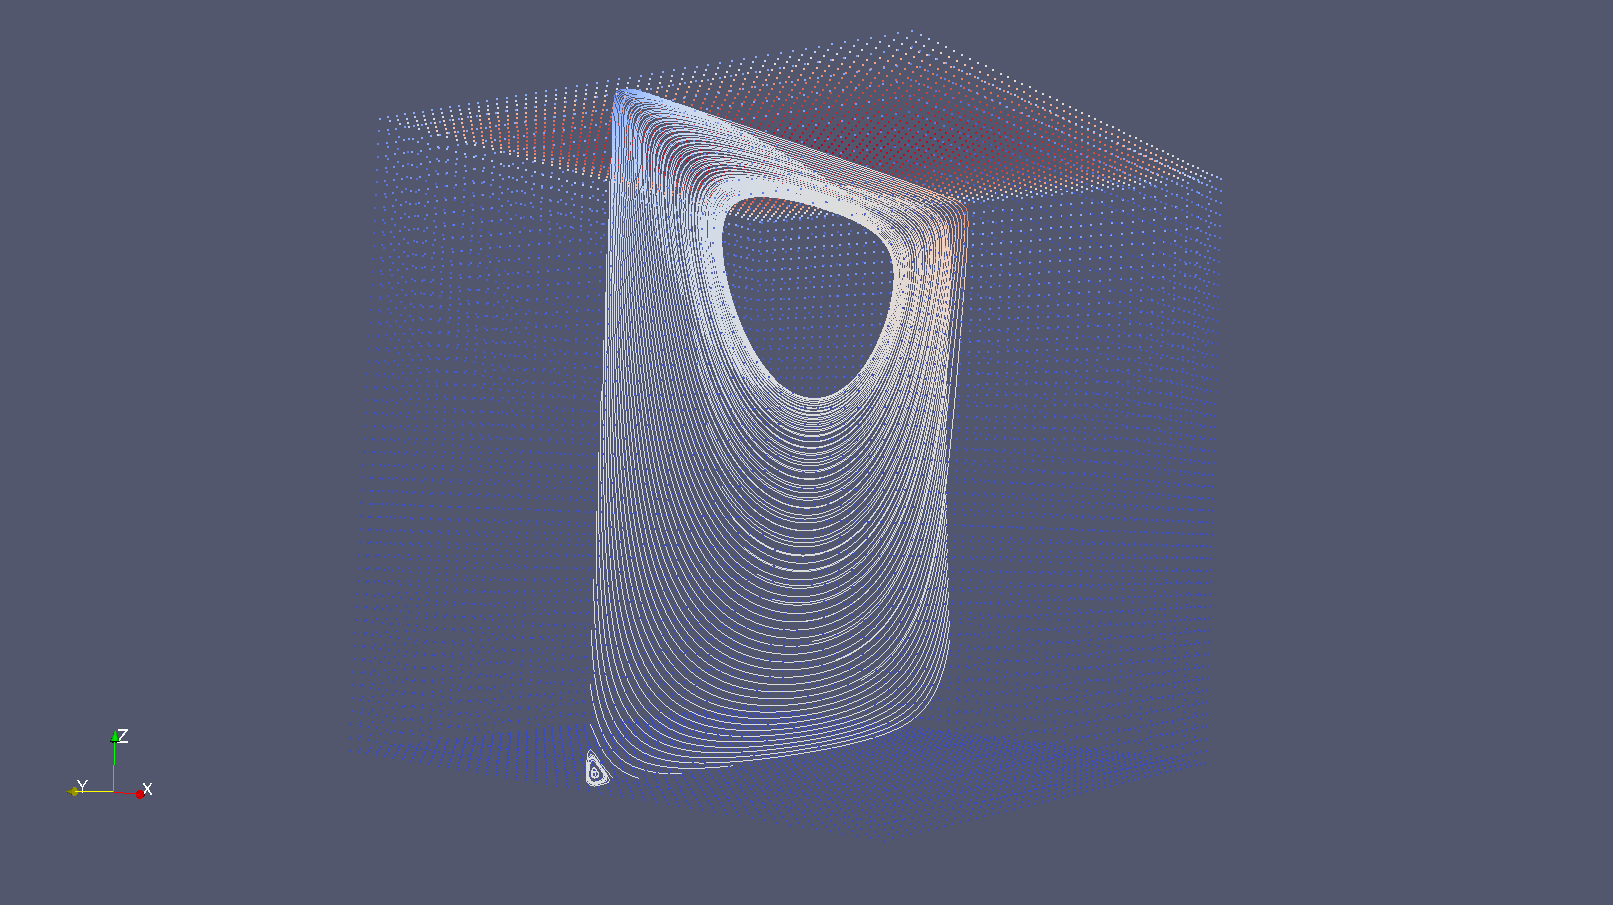
\includegraphics[width=0.7\textwidth]{img/fig10.png}
  \caption{Visualization of density of the lid-driven cavity simulation with D3Q19 model.}
\end{figure}

\begin{figure}[H]
  \centering
  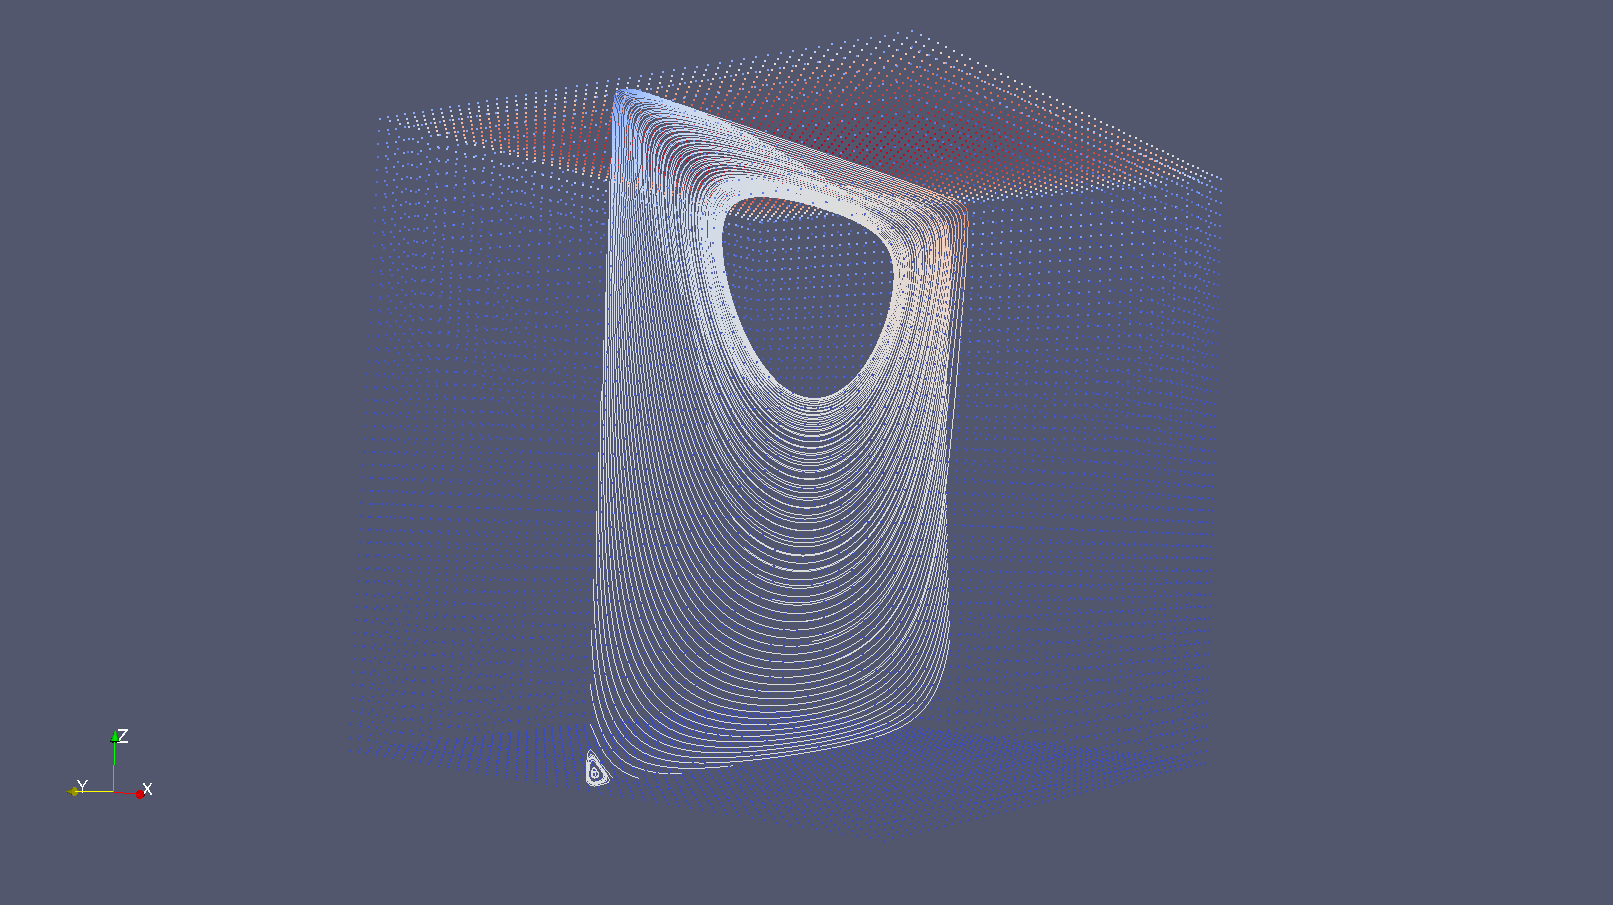
\includegraphics[width=0.7\textwidth]{img/fig11.png}
  \caption{Visualization of the velocity field and of the stream in the lid-driven cavity simulation with D3Q19 model.}
\end{figure}


\section{Own implementation: lid-driven cavity}

In my own implementation I implemented lid-driven cavity in 3D with D3Q19 model. The result of the simulation you can see on the Figure 10.

To compute streaming step and collision step I saved all $c_i$ and $t_p$ in the arrays:

\begin{lstlisting}
static const int LATTICEVELOCITIES[19][3] = {
    {0,-1,-1}, {-1,0,-1}, {0,0,-1}, {1,0,-1}, {0,1,-1},
    {-1,-1,0}, {0,-1,0}, {1,-1,0}, {-1,0,0}, {0,0,0},
    {1,0,0}, {-1,1,0}, {0,1,0}, {1,1,0}, {0,-1,1},
    {-1,0,1}, {0,0,1}, {1,0,1}, {0,1,1} };
static const double LATTICEWEIGHTS[19] = {
    1.0/36, 1.0/36, 2.0/36, 1.0/36, 1.0/36,
    1.0/36, 2.0/36, 1.0/36, 2.0/36, 12.0/36,
    2.0/36, 1.0/36, 2.0/36, 1.0/36, 1.0/36,
    1.0/36, 2.0/36, 1.0/36, 1.0/36 };
\end{lstlisting}

The main for loop looks like this:
\begin{lstlisting}
for(t = 0; t<=timesteps; t++){
    doStreaming( collide_field, stream_field,
        flag_field, xlength );
    swapFields(collide_field, stream_field);
    doCollision(collide_field, flag_field, &tau, xlength);
    treatBoundary( collide_field, flag_field,
        velocity_wall, xlength );
}
\end{lstlisting}

Function for streaming step is straightforward:
\begin{lstlisting}
void doStreaming(double *collideField, double *streamField,
int *flagField,int xlength){
  int x = 0, y = 0, z = 0;
  int i = 0;
  /* len is used to set values in lexicographic order
  "[ Q * ( z*len*len + y*len + x) + i ]" */
  int len = xlength + 2;
  /* sum of coordinates and velocity(X + Ci) */
  int sum[3];

  for(z=1; z<=xlength; z++) {
  for(y=1; y<=xlength; y++) {
  for(x=1; x<=xlength; x++) {
  for(i=0; i<Q; i++) {
    sum[0] = x - LATTICEVELOCITIES[i][0];
    sum[1] = y - LATTICEVELOCITIES[i][1];
    sum[2] = z - LATTICEVELOCITIES[i][2];

    if(sum[0]<=xlength+1 && sum[1]<=xlength+1 && sum[2]>=0 
        && sum[0]>=0 && sum[1]>=0 && sum[2]<=xlength+1) {
      streamField[ Q*(z*len*len + y*len + x) + i ] =
        collideField[Q*(sum[2]*len*len+sum[1]*len+sum[0])+i];
    } else {
      ERROR("Particles are tying to fly out of domain");
    }

  }
  }
  }
  }
}
\end{lstlisting}

The collision step function looks even nicer:
\begin{lstlisting}
void doCollision(double *collideField, int *flagField,
const double * const tau,int xlength){
  int x,y,z;
  /* len is used to set values in lexicographic order
  "[ Q * ( z*len*len + y*len + x) + i ]" */
  int len = xlength + 2;
  double density;
  double velocity[3];
  double feq[Q];
  double *currentCell;

  for(z=1; z<=xlength; z++) {
    for(y=1; y<=xlength; y++) {
      for(x=1; x<=xlength; x++) {
        currentCell = &collideField[Q*(z*len*len+y*len+x)];

        computeDensity (currentCell, &density);
        computeVelocity(currentCell, &density, velocity);
        computeFeq     (&density,velocity,feq);
        computePostCollisionDistributions(
            currentCell, tau, feq);
      }
    }
  }
}
\end{lstlisting}


\begin{figure}[H]
  \centering
  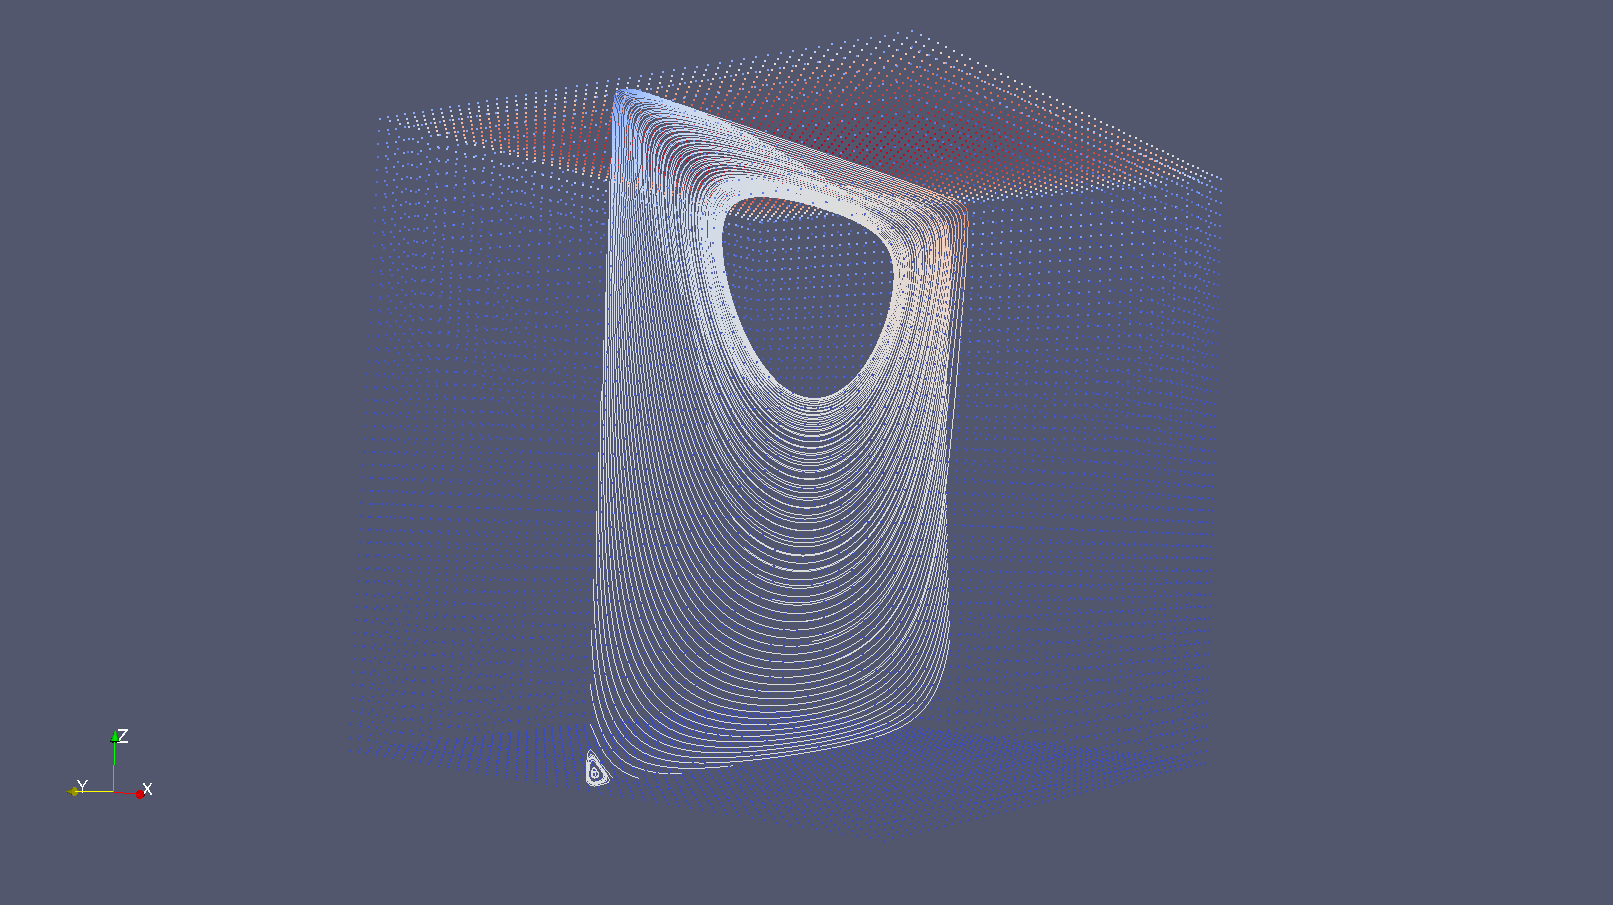
\includegraphics[width=0.7\textwidth]{img/fig10.png}
  \caption{Visualization of the lid-driven cavity simulation with D3Q19 model.}
\end{figure}


\section{Conclusion}

LBM is a quickly progressive method which is already a factor in the automotive industry. It has shown very good results in CFD. It is easy to implement but not always easy to prove it correctness (for example boundary conditions). The method is very easy to parallelize and suit very good for GPU.



\section{References}
\begin{enumerate}
\item
C. Pflaum, Simulation und wissenschaftliches Rechnen,\\
\sloppy
URL: \burl{https://www10.informatik.uni-erlangen.de/~pflaum/pflaum/SiwiR_II/skript_siwir.pdf}
\item
S. Succi, The Lattice Boltzmann Equation for Fluid Dynamics and Beyond, Oxford University Press, 2001
\item
D.A. Wolf-Gladrow, Lattice-Gas Cellular Automata and Lattice Boltzmann Models: An Introduction, Springer, 2000
\item
Article in inSIDE, Vol. 11 No. 1,\\
\sloppy
URL: \burl{http://inside.hlrs.de/_old/htm/Edition_01_13/article_06.html}
\end{enumerate}




\end{document}


